\documentclass[11pt,letterpaper]{article}
\usepackage[lmargin=1in,rmargin=1in,tmargin=1in,bmargin=1in]{geometry}
\usepackage{../style/homework}
\usepackage{../style/commands}
\setbool{quotetype}{true} % True: Side; False: Under
\setbool{hideans}{true} % Student: True; Instructor: False

% -------------------
% Content
% -------------------
\begin{document}

\homework{2: Due 09/08}{Money does not buy you happiness, but lack of money certainly buys you misery.}{Daniel Kahneman}

% Problem 1
\problem{10} Suppose that for a certain product, a company has a revenue given by $R(q)= 53.6q$ and costs given by $C(q)= 228 - 23.7q$, where $q$ is thousands of items and $R$, $C$ are measured in tens of thousands of dollars.
	\begin{enumerate}[(a)]
	\item What are the fixed costs? What are the variable costs?
	\item What is the cost production per item? How much would it cost to product 5,200~items?
	\item How much does the product sell for? What is the revenue yielded by selling 2,000~items?
	\item Find the profit function, $P(q)$.
	\item What is the smallest number of individual units of this product the company must sell to make a profit?
	\end{enumerate}



\newpage



% Problem 2
\problem{10} Ben and Jerry own an ice cream truck called `The Rolling Cones.' Each day, they drive the truck around the boroughs of NYC trying to satisfy customers in the summer heat. All the standard soft serve flavors sell for the same sale price. Once it is averaged out, the cost of the mixed used to make the cones costs approximately \$0.09 per cone. To turn a profit, they mark-up the cost per cone to \$2.00. However, the cost to run their truck and pay for upkeep, keep their vending license, and pay other associated costs is roughly \$4,235 per month. 
	\begin{enumerate}[(a)]
	\item Find Ben and Jerry's revenue function.
	\item What are Ben and Jerry's variable and fixed costs?
	\item Find Ben and Jerry's cost function. 
	\item What is the minimum number of cones that they must sell each month to turn a profit?
	\end{enumerate}



\newpage



% Problem 3
\problem{10} A local radio station charges approximately \$1,800 per advertising slot to local businesses. The building where the radio station is located costs them \$48,000 per month to rent and they pay \$18,360 in electricity each month. Additionally, the cost to pay their employees, cover health insurance, stock the office, purchase and maintain equipment, etc. is approximately \$162,000. Determine the revenue, cost, and profit functions. Then find the equilibrium point. Finally, sketch a plot of all of these in the graph below, being carefully to label your plot and indicate the equilibrium point. 
	\vfill
	\[
	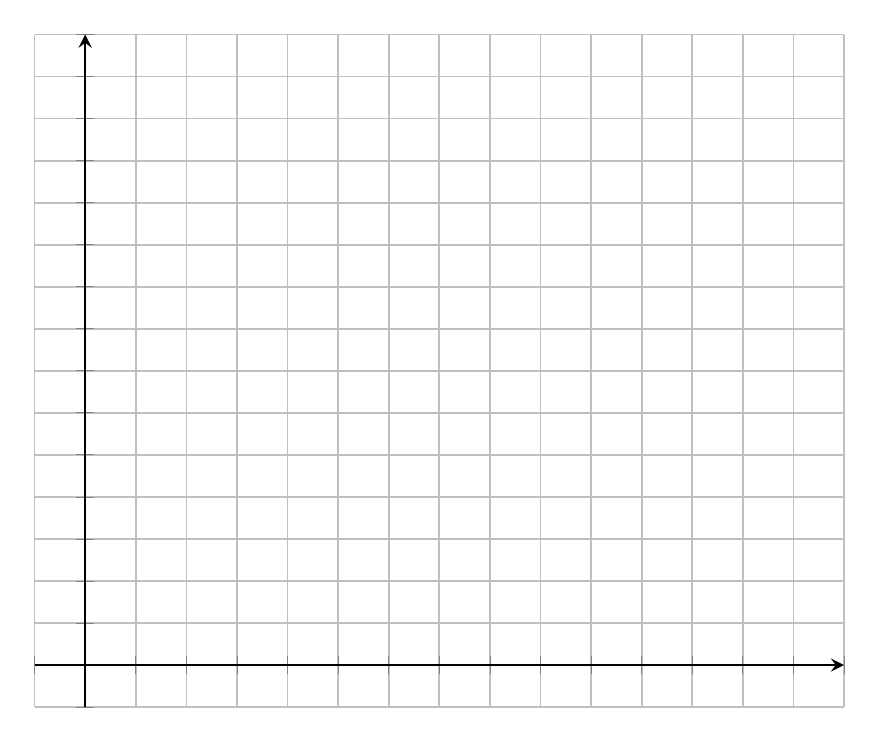
\begin{tikzpicture}[scale=1.5,every node/.style={scale=0.5}]
	\begin{axis}[
	grid=both,
	axis lines=middle,
	%ticklabel style={fill=blue!5!white},
	xmin= -1, xmax=15,
	ymin= -1, ymax=15,
	xtick={-1,0,...,15},
	ytick={-15,-14,...,15},
	xticklabels={,,},
	yticklabels={,,}
	%xlabel=\(x\),ylabel=\(y\),
	]
	\end{axis}
	\end{tikzpicture}
	\]



\newpage



% Problem 4
\problem{10} Suppose that a company has a revenue function given by $R(q)= 15.8q^2$ and cost function given by $C(q)= 3.1q^2 - 10.8q + 891$, where $q$ is measured in hundreds of items and $R$, $C$ are measured in dollars. 
	\begin{enumerate}[(a)]
	\item Find the fixed cost. 
	\item Is the marginal revenue \$15.8 per item and the marginal cost \$3.1 per item? Explain why or why not. 
	\item Find the average and marginal revenue at a production level of 1,000~items. 
	\item Find the average and marginal cost at a production level of 1,000~items. 
	\item What is the profit at a production level of 1,000~items?
	\end{enumerate}




\end{document}